\chapter{Indices and Performance Optimization}\label{sec:performance} \indexmain{performance}\indexmain{optimization}

The most important point to understand when optimizing for speed is that the expensive task is the search carried out during pattern matching. The effort for rewriting (the dominant theme in graph rewriting literature) is negligible.

Searching is carried out with a backtracking algorithm following a search plan in a fixed order, 
binding one pattern element after another to a graph element, checking if it fits to the already bound parts.
If it does fit search continues trying to bind the next pattern element (or succeeds building the match object from all the elements bound if the last check succeeds), if it does not fit search continues with the next graph element; if all graph element candidates for the currently focused pattern element are exhausted, search backtracks to the previous decision point and continues there with the next element.

Typically, first a graph element is determined with a lookup operation reaching into the graph, binding the element to a graph element of the required type (the less elements of that type exists, the better) -- then neighbouring elements are traversed following the graph structure (the less neighbouring elements exists, the better), until a match of the entire pattern is found.


%%%%%%%%%%%%%%%%%%%%%%%%%%%%%%%%%%%%%%%%%%%%%%%%%%%%%%%%%%%%%%%%%%%%%%%%%%%%%%%%%%%%%%%%%%%%%%%%
\section{Search Plans}

A search plan for the pattern in figure \ref{perf:figpatterntosearch} is:\\
\texttt{lkp(v1:A); out(v1,e1:a); tgt(e1,v2:B); out(v2,e3:b); tgt(e3,v3:C); out(v3,e2:a)}\\
The search operations \texttt{lkp} denotes a node (or edge) lookup in the graph, \texttt{out} follows the outgoing edges of the given source node and \texttt{in} follows the incoming edges ot the given target node, while \texttt{src} fetches the source from the given edge and \texttt{tgt} fetches the target from the given edge.

For some graphs the search plan might work well, but for the graph given in figure \ref{perf:figgraphtosearchin} it is a bad search plan.
Why so can be seen in the search order sketched in figure \ref{perf:figbadsearch}.
Due to the multiple outgoing edges of \texttt{v1} of which only one leads to a match it has to backtrack several times.

This schedule in contrast is a a good one:\\
\texttt{lkp(v3:C); out(v3,e2:a); tgt(e2,v2:B); out(v2,e3:b); in(v2,e1:a); src(e1,v1:A)}\\
corresponding to the search order depicted in figure \ref{perf:figgoodsearch}.

It is crucial for achieving high performance to prevent following graph structures splitting into breadth as given in this example, and especially to avoid lookups on elements which are available in high quantities.

\begin{figure}[p]
  \centering
  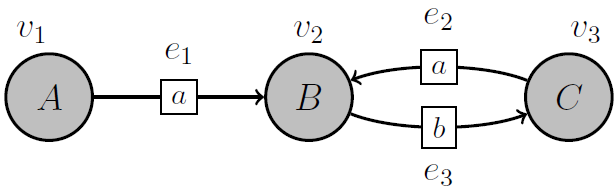
\includegraphics[width=0.7\textwidth]{fig/Pattern}
  \caption{Pattern to search}
  \label{perf:figpatterntosearch}
\end{figure}

\begin{figure}[p]
  \centering
  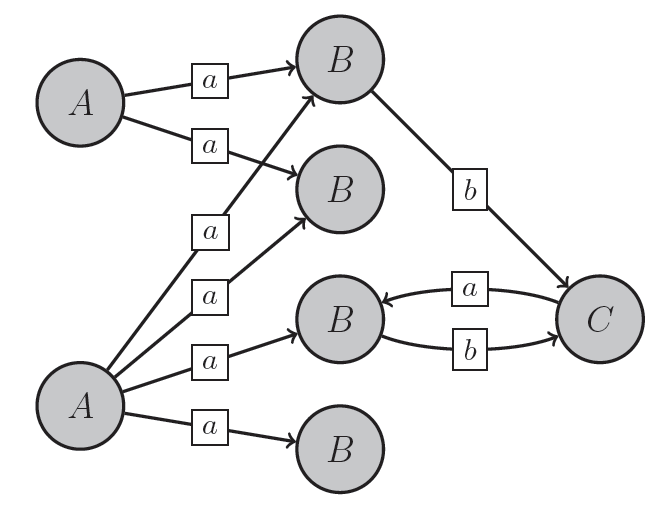
\includegraphics[width=0.7\textwidth]{fig/Graph}
  \caption{Host graph to search in}
  \label{perf:figgraphtosearchin}
\end{figure}

\pagebreak

\begin{figure}[p]
  \centering
  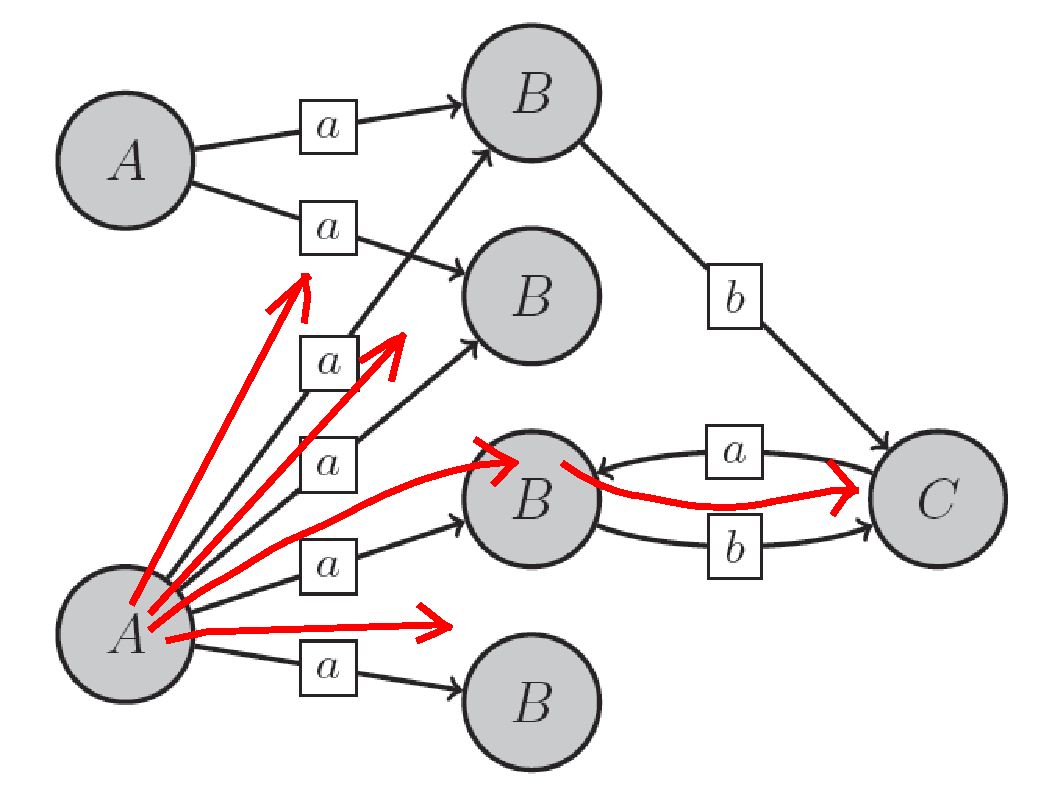
\includegraphics[width=0.7\textwidth]{fig/GraphBad}
  \caption{Bad search order}
  \label{perf:figbadsearch}
\end{figure}

\begin{figure}[p]
  \centering
  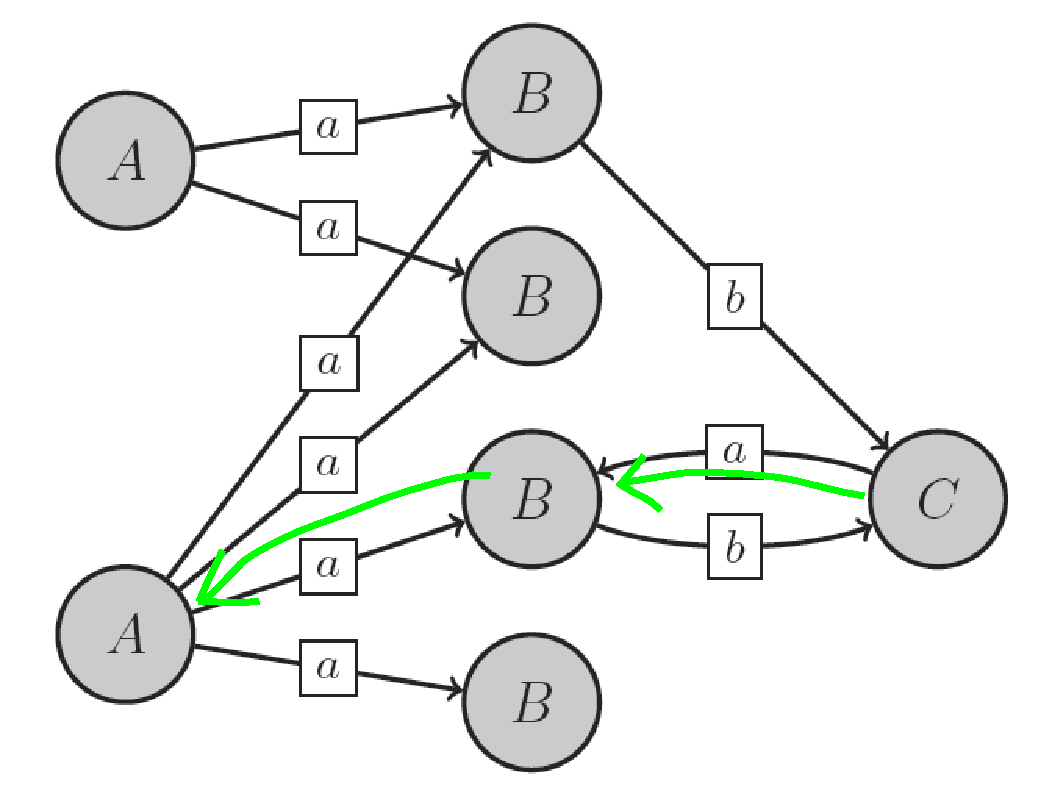
\includegraphics[width=0.7\textwidth]{fig/GraphGood}
  \caption{Good search order}
  \label{perf:figgoodsearch}
\end{figure}


%%%%%%%%%%%%%%%%%%%%%%%%%%%%%%%%%%%%%%%%%%%%%%%%%%%%%%%%%%%%%%%%%%%%%%%%%%%%%%%%%%%%%%%%%%%%%%%%
\section{Find, Don't Search}
Better than searching for elements with certain characteristics, 
traversing each and every node or edge in the graph, 
subjecting it to a test for the characteristic,
is to find them straight ahead without search,
utilizing a data structure that allows to tell the elements that follow the characteristic apart from the ones that do not.
Welcome to indices as known from database parlance.
In \GrG{} they following types of indices are supported:
\begin{enumerate}
	\item Type indices
	\item Neighbourhood indices
	\item Attribute indices
	\item Incidence count indices
	\item Name index
	\item Uniqueness index
\end{enumerate}

%-----------------------------------------------------------------------------
\subsection{Type Indices}
All the nodes or edges in \GrG{} of a certain type are contained in a list that can be acessed in $O(1)$ and iterated in $O(k)$ with $k$ being the number of elements in that list (the nodes or edges of same type), in contrast to $n$, being the number of nodes or edges in the graph.
The first node or edge in a pattern is typically bound by iterating such a type list.
In case the pattern is disconnected, a lookup is needed per connected component.
In case multiple types have very few members, the search planner may decide to use several lookups even in case of a connected pattern.
(This can be especially the case for reflexive marker edges pointing to the current point of processing/focus of attention in the graph.)

%-----------------------------------------------------------------------------
\subsection{Neighbourhood Indices}
All the edges outgoing from a node are contained in a list that can be accessed in $O(1)$ and iterated in $O(k)$ with $k$ being the number of elements in that list (the outgoing edges), in contrast to $n$, being the number of edges in the graph.
All the edges incoming to a node are contained in a list that can be accessed in $O(1)$ and iterated in $O(k)$ with $k$ being the number of elements in that list (the incoming edges).
So following neighbouring elements, crawling alongside the structure is very cheap in \GrG{ } -- and possible in both directions, following the edges as well as in their opposite direction.

It is cheap in graph databases, too, but absolutely not in relational databases.
To follow a relation, there you have to join two complete tables, building the cartesian product of two tables (materializing only the rows where they agree) -- you must inspect all edges in the graph to find the neighbours.
Typically you optimize this with a database index that allows to find the elements of the second table matching your focused element of the first table in $O(log(n))$ -- but for large $n$ or for complex queries this global product is way less efficient than direct local access to exactly the neighbouring elements.
(Furthermore, a table join is conceptionally and notationally much heavier than an edge in a graph pattern).

In case of undirected edges, or arbitrary directed edges in the pattern, both directions are searched,
both lists -- the outgoing list as well as the incoming list -- are crawled.

%-----------------------------------------------------------------------------
\subsection{The Costs}\label{sec:performancememory} 
The type and neighbourhood indices are built into each and every \GrG{} graph, wired into a system of ringlists (cf. \ref{sec:generatedcode}).
They are implicitly used by \GrG{}, pattern matching is just carried out alongside them, in an order decided upon by the search planner. 
You always benefit from them during matching (most if you are using statistics-based search planning), but you must always pay their price:
The memory consumption of a \GrG{} node without attributes is 36 bytes using a 32bit CLR (5 pointers a 4 bytes, a 4 bytes flags field/bitvector, a 4 bytes unique id field, plus 8 bytes .NET object overhead), it is 64 bytes for a 64bit CLR (5 pointers a 8 bytes, a 4bytes flags field, a 4 bytes unique id field, plus 16 bytes .NET object overhead).
The memory consumption of a \GrG{} edge without attributes is 52 bytes using a 32bit CLR (9 pointers a 4 bytes, a 4 bytes flags field/bitvector, a 4 bytes unique id field, plus 8 bytes .NET object overhead), it is 96 bytes for a 64bit CLR (9 pointers a 8 bytes, a 4 bytes flags field, a 4 bytes unique id field, plus 16 bytes .NET object overhead).
Attributes are cheap, they only increase this by the .NET-memory-footprint of their underlying objects.
The runtime price of those indices during graph manipulation is low, adding a graph element is done in $O(1)$, removing a graph element is done in $O(1)$, too. 
(Furthermore, those indices allow to optimize loops by starting matching of the next iteration where the previous iteration left of (search state space stepping -- a further built-in contribution to the motto "Find, Don't Search")).
We consider this the best you can get for the task of efficient pattern matching on typed, attributed multigraphs -- those indices are simply worth their price in the general case (you can only improve on this by exploiting the specifics of a less general graph model or by restricting yourself to less general and non-automatic pattern matching).

%-----------------------------------------------------------------------------
\subsection{Consequences For Optimization}

\subsubsection*{Use types!}
Fine grain types cause a fast lookup of the first pattern element(s), or more exactly: they cause a small list of candidate elements for the first pattern element to be tried.
And they cause quicker pruning of search branches because of early failing type checks.
Using fine-grain types is easy in GrGen, for multiple inheritance on node and edge types (cf. \ref{nodeandedgetypes}) is supported.
Besides, the more fine grain the graph is typed, the better are the statistics, allowing \GrG{ } to find better search plans (see more for this below).

\subsubsection*{Prune early}
Attribute conditions are evaluated as soon as all needed graph elements are matched (saving us from enumerating futile match extensions).
But the unit of scheduling are the full attribute condition expressions. 
If an expression can be separated into different parts that depend on less pattern elements than the entire expression (such a separation is trivial for boolean expressions joined by logical conjunctions), split it into those parts.
The parts are then checked earlier in the search process.
You could even introduce checks that are logically not needed because a later check removes all incorrect matches anyway, just to achieve better performance, which is the case if the checks allow to prune some branches from the search space earlier.
This holds as long as the checks are cheap, if they are expensive you could do the opposite and introduce artificial dependencies to all pattern elements instead, to ensure the attribute condition is evaluated as late as possible.

\pagebreak

\subsubsection*{Prefer directed edges}
Non-directed edges in the pattern are searched in both directions, considerably increasing the search space.
Use non-directed edges only if they you really needed them.
For some problems this is the case, you then simply have to pay the price of the increased effort for the symmetry.
But some problems where undirected edges are more natural can be easily encoded with directed ones -- in case of performance problems, refactor and optimize them to employ only directed edges, imposing an arbitrary but deterministic direction on the edges.
Besides, the vstructure statistics are more discriminating in case of directed edges, leading to better search planning results; in case of undirected ones the information from both directions is coalesced.

%\pagebreak

\subsubsection*{Beware of Disconnected Patterns}
Disconnected patterns cause a combinatorial explosion of the matches, because the overall number of matches equals the cartesian product of the partial matches of the disconnected parts. 

This is inevitable and a price that must be simply paid if this is really needed.
But it is normally not needed, and, most important, is not specified accidentally, as a disconnected pattern in single flat pattern is typically immediately visible.
But take care of nested patterns or subpatterns.
You might overlook that nested patterns and subpatterns are matched strictly one after the other and especially after their containing pattern.
You cannot ignore block borders and subpattern calls, they disconnect otherwise connected components.
Esp. take care of not disconnecting patterns when factoring out a common part into a subpattern to improve the code.
But due to inlining, things look better than what was said until now.

\begin{example}
Take a look at pattern nesting, when the pattern is disconnected, you run into issues due to combinatorial explosion.
This holds for sure for alternative and iterated patterns.

So you must take care of pattern cardinality ...
\begin{grgen}
test bad {
	n1:Node; n2:Node; // builds cartesion product of all nodes in the graph (O(n*n))
  multiple {
		n1 --> n2; // then filters it down to the connected nodes
  }
}
\end{grgen}
... and alternatives ...
\begin{grgen}
test bad {
	n1:Node; n2:Node; // builds cartesion product of all nodes in the graph (O(n*n))
  alternative {
		single {
			n1 --> n2; // then filters it down to the connected nodes
		}
  }
}
\end{grgen}
\end{example}

\begin{example}
Take a look at pattern nesting, when the pattern is disconnected, you run into issues due to combinatorial explosion.
This may hold for independent and subpatterns -- but inlining is of help here.

The edge from the independent in the example is typically inlined into the pattern removing the issue...
\begin{grgen}
test bad {
	n1:Node; n2:Node; // builds cartesion product of all nodes in the graph (O(n*n))
  independent {
		n1 --> n2; // then filters it down to the connected nodes
  }
}
\end{grgen}
... as is the subpattern body inlined into the pattern, removing the performance issue.
\begin{grgen}
test bad {
	n1:Node; n2:Node; // builds cartesion product of all nodes in the graph (O(n*n))
  :P(n1,n2);
}
pattern P(n1:Node, n2:Node) {
	n1 --> n2; // then filters it down to the connected nodes
}
\end{grgen}
Take a look at the output of the \texttt{explain} command to check whether inlining occured.
\end{example}

The need to take nested pattern borders and subpattern calls into account is due to the recursive descent matching with a multi-pushdown machine as described in Section \ref{matchingflow} and Section \ref{pushdownmachine}.

Subpatterns are matched top-down, from the input parameters on.
If the input arguments are disconnected in the pattern containing the subpattern, the containing pattern enumerates the cross product of the matches of the disconnected parts, which is only later on filtered for the ones which are connected.
This will likely wreak havoc on the search performance.
Even if you don't search for all matches, if you only compute a single overall match --- the calling pattern must enumerate a lot of combinations of its parts (worsened by the fact that those are typically found oftenly because of their simplicity), until the nested pattern finally is able to connect one of the disconnected pairs fed into it.
It might be more efficient to just search from a start parameter towards a connected end location, and yield the found one out (cf. \ref{sec:localvarorderedevalyield}), or to search from a start parameter all connected end locations, collecting the found ones in a result set; and then to check the ones found alongside connectedness in a second step.

Nested patterns are matched top-down, from the input parameters on, just that parameter passing is implicit there, the elements from the containing pattern which are referenced in the nested pattern are passed in automatically as arguments.
The holds especially for the \texttt{alternative} and \texttt{iterated} constructs which are matched with the pushdown machine (cf. \ref{pushdownmachine}), too, but also for the \texttt{negative} and \texttt{independent} constructs which are matched with nested local code embedded into the matcher code of their containing pattern.

But don't shy away from using subpatterns or independents too easily, \indexed{inlining} is helping here!

The elements from an independent that are linking a disconncted pattern are typically inlined into their using pattern.
The elements from a subpattern are often inlined into their using pattern, causing the pattern to get connected (again), 
but also removing the pushdown machine overhead.
But you must take into account that the \emph{inlining} implemented in GrGen is limited to depth one.
If a pattern is disconnected over two or more levels of subpattern usage (which might happen statically with one subpattern using another subpattern, and will for sure dynamically on a subpattern recursion path), it will hit performance.
You may have a look at the output of the \texttt{explain} command (cf. \ref{custom}) to see if the subpatterns are disconnected; this is typically indicated by multiple lookups in the containing pattern, and the fact that the starting points passed as preset parameters to the nested or subpatterns get connected only there with search commands.


%-----------------------------------------------------------------------------
\subsection{Search Planning On Request}
Search planning at runtime is only carried out on request!
You must analyze the graph and then re-generate the matchers at runtime,
with \texttt{custom graph analyze} and \texttt{custom actions gen\_searchplans} (issued on the command line or to the \texttt{Custom}methods of the graph and the actions objects);
you may have a look at the effects of replanning with the \texttt{custom actions explain <actionname>} command.
See subsection \ref{custom} for more on this.

The initial static search plans start with a lookup of an arbitrary edge, and then arbitrarily follow graph structure.
Interestingly, in many cases this still works quite well because of the quick pruning of the type checks in a well-typed graph.
In addition, often the rules work from some parameter nodes onwards, which are typically well suited start points for search.

You can inspect the current search plan employed wit the explain command.
Use it before search planning to inspect the statically generated search plans.
Use it afterwards to inspect how the elements are matched then.

Beware: the analyze command is not for free, it visited all the nodes and edges in the graph, computing for each start node of a $(NodeType, EdgeType, NodeType)$-triple the number of edges of the edge type leading to an end node of the end node type -- for all node and edge types known.
Given that information search planning can compute a search plan that avoids structures splitting into breadth (V-structures);
given the information about the element counts per type (which is directly available from the host graph), 
search planning can avoid lookups on populated types.
This typically leads to the best results, but not always -- sometimes you may fare better by manually assigning priorities to the pattern elements, thus influencing the search order of the initial static search plan (high-prio elements are matched first) -- if you don't re-generated the search plan for that rule at runtime the static search plan is kept in place.

Again: Use types!
The more fine grain a graph is typed, the better are the statistics regarding the splitting factors (V-Structures) and the number of elements of a certain type, and the better are then in consequence the search plans in their ability of evading splitting structures and avoiding lookups of oftenly occurring types.

%-----------------------------------------------------------------------------
\subsection{Attribute Indices}
In addition to the built-in type and neighbourhood indices, you may declare attribute indices.
An attribute index allows to do a lookup based on an attributes value, or a range of attribute values.
This stands in contrast to the default behaviour of carrying out a lookup on the type, visiting all $n$ elements of the type, filtering them down to the elements of interest (within range) with an attribute condition.
If this means you have to inspect a lot of values while searching only for a few ones, you should use an attribute index and benefit from its massively improved selectiveness for the lookup.
It requires only $O(log(n))$ to search for the first element, and $O(k)$ for the $k$ elements within the bounds specified.
It is implemented with a balanced binary search tree (an AA-tree\cite{Andersson93balancedsearch} to be exact) that requires three pointers plus one 4 byte integer per element contained in the index (two pointers to the left and right tree nodes, and one to the graph element as value), which is really cheap.
But it must be maintained on graph changes, which is less cheap.
On each and every graph element insertion and removal, but esp. attribute assignment, the index needs to be updated, which is an $O(log(n))$ operation.
That's only logarithmic, but clearly worse than the default $O(1)$ behaviour of \GrG{}, so if you do a lot of graph manipulations and only few lookups based on it, an index may in fact degrade performance.

\subsubsection*{Declaration in the model}
In contrast to type and neighbourhood indices which are always available (they define the core of a \GrG{}-graph) and are implicitly used (by matching the specified pattern), all other indices must be worked with explicitly.

An attribute index must be declared in the model.

\begin{rail}
  AttributeIndexDecl: 'index' IndexName lbrace Type '.' AttributeName rbrace;
\end{rail}\ixnterm{AttributeIndexDecl}

Following the \texttt{index} keyword, a name for the index is specified; in the body of the index, the type and name of the attribute to be indexed are given.

\subsubsection*{Usage in the rules}\label{sub:indexusage}

In the pattern part you may ask for an element to get bound to an element from an index;
this is syntactically specified by giving the index access enclosed in left and right braces after the element declaration.
If the type of the element retrieved from the index is not compatible to the type of the pattern element specified,
or if the index is empty, matching fails.
The elements from the index are successively bound to the pattern element, then the rest of the pattern is bound and checked, until the requested number of matches is found.

\begin{rail}
  IndexAccess:
    lbrace IndexName '==' Expression rbrace |
		lbrace ('ascending'|'descending') '(' (IndexBound (',' IndexBound)?)? ')' rbrace;
	IndexBound: IndexName ('<'|'<='|'>'|'>=') Expression;
\end{rail}\ixnterm{IndexAccess}

The pattern element may be bound to the elements from the index with an attribute value equal to a specified value,
or to the elements from the index in ascending or descending order.
In case of ordered access, you may specify no bound, this is typically only of interest when only one match is requested, the one with the highest or lowest attribute value (satisfying the other constraints of the pattern), or you may specify a lower or an upper bound, or you may specify a lower \emph{and} an upper bound.

\begin{rail}
  IndexAccessLoopStatement:
    ForIndexAccessHeader lbrace (Statement*) rbrace;
  ForIndexAccessHeader:
    'for' '(' Var ':' GraphElementType 'in' IndexAccess ')';
  IndexAccessLoopSequence:
    'for' lbrace Var ':' GraphElementType 'in' IndexAccess ';' RewriteSequence rbrace;
\end{rail}\ixnterm{IndexAccessLoopStatement}\ixnterm{IndexAccessLoopSequence}

The index can be accessed furtheron from the statements of the rule language in the form of a loop.
The \emph{IndexAccess} in the loop header follows the format used in the index access in the pattern.
The iteration variable is bound to the graph element retrieved from the index, for each such element, then the body is executed for each such element.
Moreover, the index can be iterated over in the sequences.

%-----------------------------------------------------------------------------
\subsection{Incidence Count Indices}
Attribute indices can be seen as a general-purpose device, that extends the built-in ability of quick lookup by-type and of quick lookup by-neighbourhood with a quick lookup by-attribute, thus giving complete quick-lookup coverage for all foundational elements of the graph model.
Incidence count indices in contrast are more of a special-purpose device for a certain abstraction that can applied to the graph -- the \emph{count} of incident edges -- and are benefitial only if that abstration is of importance.
They allow you to quickly lookup nodes based on their number of incident edges.
This is benefitial if you need to quickly fetch nodes with a certain number of incident edges;
but especially for algorithms that work best when starting with the nodes with the highest number of incident edges, going downwards, or vice versa.

The index furtheron allows to fetch the incidence count for a node quickly with just an index lookup, 
but typically no considerable gains can be made from this, as counting the incident edges of a node is commonly cheap (an $O(log(n)$ index lookup versus an $O(k)$ counting enumeration, with $k$ being the number of edges incident to the focused node).

\subsubsection*{Declaration in the model}

An incidence count index must be declared in the model.

\begin{rail}
IncidenceCountIndexDecl: 'index' IndexName lbrace IncidenceFunction rbrace;
IncidenceFunction: 
  IncidenceFunctionName '(' NodeType ')' |
  IncidenceFunctionName '(' NodeType ',' EdgeType ')' |
  IncidenceFunctionName '(' NodeType ',' EdgeType ',' NodeType ')'
  ;
\end{rail}\label{IncidenceCountIndexDecl}

Following the \texttt{index} keyword, a name for the index is specified; in the body of the index, the incidence function and its types are given.
The admissible incidence functions are \texttt{incident}, \texttt{incoming}, and \texttt{outgoing}, with their obvious meanings (as already introduced in \ref{sub:querybyneighbourhood}).
The count of the edges complying to the specified incidence function is indexed, for all nodes in the graph of the type of the first node in the incidence function.

\subsubsection*{Usage in the rules}
An incidence count index can be used in the pattern in exactly the same way as an attribute index, see above \ref{sub:indexusage}.

In addition to the index lookup in the pattern, 
the count may be queried from the rule language expressions (the attributes can be accessed directly for a pattern element, the incidence count would have to be counted in contrast, but this only saves time for heavily connected nodes).

\begin{rail}
  IncidenceCountIndexAccessExpr:
    IndexName '[' Expression ']';
\end{rail}\ixnterm{IncidenceCountIndexAccessExpr}

The index access specfied in indexer notation expects a node (of the type as specified with the first node type in the incidence function) as input argument, and returns the incidence count for that node as stored in the index as \texttt{int}.

%-----------------------------------------------------------------------------
\subsection{Name Index}\label{sec:nameindex}
A named graph is a graph where each element bears a unique name and can be looked up quickly by that name.
So basically it works as a graph with an integrated key-value store from a string to graph elements; and from graph elements to their string.
It is implemented with two hash maps, one from the name to the elements, and the other from the elements to the name.
Lookup is carried out in $O(1)$ (either way).
Maintaining the index on graph insertions and removals is carried out in $O(1)$, too.
So in contrast to the attribute index and the incidence count index, a name index does not allow multiple elements per indexed property (which is here the name).

\subsubsection*{No declaration needed}
The name index does not need to be declared, it is implemented with the named graph, which is always generated together with its sibling, the non-named graph.
If you are working with the Shell, this is the only kind of graph you'll be working with, as the shell always instantiates the named graph (it delivers the \emph{persistent names} you see in the debugger).
At API level you may opt for the non-named graph that is considerably cheaper regarding memory usage -- a named graph requires not much less than about twice the amount of memory of a plain graph.
But please note that the export and import capabilities require uniquely named elements and thus only work with named graphs.
If given a plain graph the exporters just create a named graph, and a graph is always read in as a named graph.
So non-named graphs are typically only of interest if you don't need to persist them into a serialization format.

\subsubsection*{Usage in the rules}
The name index can be used in the pattern to lookup graph elements by their name, with the same syntax as used in the Shell for accessing elements by their (persistent) name.

\begin{rail}
  NamedIndexAccessExpr:
    lbrace '@' '(' Expression ')' rbrace;
\end{rail}\ixnterm{NamedIndexAccessExpr}

There is at most one element existing with the name asked for; if no graph element with that name exists, matching fails and backtracks, if an element exists, the pattern element is bound to it, and matching continues.
Please note that the (string-)expression used to compute the name is only allowed to reference at most one other pattern element (not handed in as parameter).

The name index may be further queried from the rule language expressions with 3 functions:
\begin{description}
\item[\texttt{nameof(.)}] returns the name (type string) of the given node or edge (or (sub)graph, a missing argument amounts to the host graph).
\item[\texttt{nodeByName(.)}] returns the node of the given name, or null if no node of that name exists.
\item[\texttt{edgeByName(.)}] returns the edge of the given name, or null if no edge of that name exists.
\end{description}

The names are normally automatically assigned (computed from a global counter increased with each element, prepended by the dollar symbol -- unless you specify a name with an attribute initialization list, cf.\ref{sec:attribinitrule}), but you may assign a different name to an attribute element.
This can be only done in an \texttt{eval}-block, or a \texttt{procedure}, with a \texttt{nameof}-assignment.

\begin{rail}
  NameofAssignment:
    nameof '(' Element ')' '=' Expression;
\end{rail}\ixnterm{NameofAssignment}

When you do so, it is your responsibility to ensure the name does not already exists, otherwise the assignment will cause a runtime exception.
The same syntax may be used to assign the name of a (sub)graph, a missing element amounts to the host graph.

%-----------------------------------------------------------------------------
\subsection{Uniqueness Index}\label{sec:uniqueness}
Uniquness can be applied in two parts, the i) uniqueness \emph{constraint}, and ii) the uniqueness \emph{index}.
The uniqueness \emph{constraint} ensures that each element in the graph has a unique id. 
But only for a given graph element can the unique id be obtained.
You may see it as a key-value store from graph elements to their ids -- it is a very efficient one, as the unique-id is stored in the graph elements. 
The uniqueness \emph{index} ensures in addition that you can fetch a graph element by its unique id, extending the uniqueness property to an index allowing for quick graph element lookup.
You may see it as a key-value store from the unique ids to their graph elements.
This one is realized with an array of unique ids to graph elements.
So lookup is carried out efficiently in $O(1)$ either way.
Maintaining the uniqueness information is somewhere between $O(1)$ and $O(log(n))$, as the ids of deleted elements have to be stored in a heap (the data structure, not the memory model) for quick reuse of the lowest one (this way we ensure a maximally packed id range, which is of importance to keep the index array and the is-matched-bit-arrays of the parallelized matchers small and packed).
A uniqueness index does not allow multiple elements per indexed property (which is here the unique id), like the name index, and in contrast to the attribute and incidence count indices.

\subsubsection*{Declaration in the model}
The space for the unique id is always reserved in the graph elements, but only if an uniqueness constraint is declared is it really filled with unique ids (and in case when you declare another index in the model, as they depend on the unique ids, and in case you use parallelize annotations, as the parallelized matchers depend on the unique ids, too).
If you need to fetch graph elements by their unique ids, you must declare an unique index (in addition or instead).

\begin{rail}
  UniqueConstraintDecl: 'node' 'edge' 'unique' ';';
  UniqueIndexDecl: 'index' 'unique' ';';
\end{rail}\ixnterm{UniqueConstraintDecl}\ixnterm{UniqueIndexDecl}


\subsubsection*{Usage in the rules}
The unique index can be used in the pattern to lookup graph elements by their unique id.

\begin{rail}
  UniqueIndexAccessExpr:
    lbrace 'unique' '[' Expression ']' rbrace;
\end{rail}\ixnterm{UniqueIndexAccessExpr}

There is at most one element existing with the unique id asked for; if no graph element with that unique id exists, matching fails and backtracks, if an element exists, the pattern element is bound to it, and matching continues.
Please note that the (int-)expression used to compute the unique id is only allowed to reference at most one other pattern element (not handed in as parameter).

The unique constraint may be further queried from the rule language expressions with the \texttt{uniqueof} function,
the unique index with the \texttt{nodeByUnique} and \texttt{edgeByUnique} functions:
\begin{description}
\item[\texttt{uniqueof(.)}] returns the unqiue id (type int) of the given node or edge (or (sub)graph, a missing argument amounts to the host graph).
\item[\texttt{nodeByUnique(.)}] returns the node of the given unique id, or null if no node of that unique id exists.
\item[\texttt{edgeByUnique(.)}] returns the edge of the given unique id, or null if no edge of that unique id exists.
\end{description}

The unique ids are automatically assigned (from a global counter increased with each element, but reusing already handed out ids that return to the pool once their element is removed from the graph). In contrast to the names you cannot change the id assignment.


%%%%%%%%%%%%%%%%%%%%%%%%%%%%%%%%%%%%%%%%%%%%%%%%%%%%%%%%%%%%%%%%%%%%%%%%%%%%%%%%%%%%%%%%%%%%%%%%
\section{Location passing and memorization}
Often in a transformation you know the location that needs processing from a previous step.
In this case, return these locations out from the rules, store them in variables of node (or edge) type, and hand them in again via rule arguments to the follow-up rules.
Or call embedded rules, directly handing elements from the rule, saving you the intermediate assignments.

Commonly, this is just the right way of handling this situation, 
as you must continue processing the very spot you just processed with the previous rule(s) to achieve a valid result.
Sometimes you don't need to, but gain higher performance when you do so.
Optimize this way then, use \emph{rooted} pattern matching, with roots defined by previous rules, it's cheaper as it saves you the lookup in the graph.
A different way of parameter passing is adding reflexive edges to the graph to mark the spot of processing.
This is normally working well, too, but the parameter passing is typically easier and does not "pollute" the graph with processing information.

In case of a statically not known number of locations as they appear e.g. in wavefront algorithm, you may store the locations in storages (cf. chapter \ref{cha:container}), i.e. collection valued variables (which are iterated over in the sequences or passed to the rules as \texttt{ref} parameters).
Search will then start from these parameters, instead of a looking up a value in the graph by type (unless search planning taking the statistics about the graph into account comes to the conclusion that a lookup on a super-seldom type is still the better approach).

A sophisticated way of remembering facts about non-local properties is to computed them with data flow analyses (see section \ref{subsub:flow}) and store them as attributes in the graph elements.
This allows to replace searching for distant values, or global properties like reachability, by checking a local property, at the price of re-running an analysis every time the graph changes in an important way.

With variables and storages you build indices into the graph, indices which are typically more selective than the automatically supplied indices; 
but in contrast to the automatically built ones, you must maintain them by hand.

The approach of remembering state instead of searching when needed has a clear caveat: the code becomes susceptible to ordering effects (more brittle), it may become less readable. As in normal programming, you must balance performance optimizations against maintainability.


%%%%%%%%%%%%%%%%%%%%%%%%%%%%%%%%%%%%%%%%%%%%%%%%%%%%%%%%%%%%%%%%%%%%%%%%%%%%%%%%%%%%%%%%%%%%%%%%
\section{Profile and Parallelize}\label{sec:performanceparallel}

A basic and often sufficient means of profiling is built-in into GrShell:
After each sequence execution the time required to carry it out is printed.

Sometimes you need further information about what's going on.
Use the built-in profiling then (you may of course apply a profiler on the generated code, but then you descend to the level of implementation of \GrG).

You can do so by specifing the \texttt{profile} compiler option (cf. \ref{grgenoptions}) to request search code instrumentation, or better the \texttt{set profile on} shell command (cf. \ref{sec:compilerconfigshell}).
You will receive two kinds ouf results when executing matchers instrumented that way.

\begin{enumerate}
	\item After each sequence execution, the shell will print out the number of search steps that occured, in addition to the time. A search step consists of binding a graph element to a pattern element.
	\item You can request a detailed per-action profile with the \texttt{show profiles} shell command (cf. \ref{grsthings}).
\end{enumerate}

The detailed per-action profile contains a value that gives you a hint about the expected use of matcher parallelization, the higher the number the better is the rule suited.

\subsubsection*{Parallelize}
A rule or test annotated with \texttt{[parallelize=k]} will be matched with \texttt{k} worker threads from a thread pool.
More exactly: at most \texttt{k} worker threads, the number is clipped by the number of really available processors, on a single core the normal sequential matcher will be used.
(The current implementation defined maximum is 64.)

Parallelization distributes work alongside the first loop that is binding a pattern element to candidate graph elements.
If that loops only once nothing is gained.
If each loop iteration only executes very few search work following candidate assignment,
things become \emph{slower} because of threading and locking overhead.
Don't just append the parallelize annotation to each and every rule in the hope things will become faster!
Only search intensive-tasks benefit, only for them the overhead of parallelization pays off.
But for those search-intensive tasks, you can achieve high speedups, reaping benefits from our-days multicore machines. 

Remark: Only the pattern matcher of an action is parallelized, so only the search process is parallelized.
This offers the biggest bang for the bucks invested, as search is \emph{the} expensive task, and it allows you to stick to the much simpler sequential programming model.
A parallelization of the kind presented in \cite{ParGraErs} offers potentially even higher speedups, but at the price of dealing with a parallel programming model, and at the price of graph partitioning that is very hard to get right in a general-purpose tool.

There's a second part that can be parallelized, the \texttt{equalsAny} function checking for graph isomorphy of a new candidate against a set of known graphs.
The \emph{EqualsAnyParallelization} clause in the model must specify the number of worker threads used in parallel.
A \verb#for equalsAny[parallelize=8];# requests 8 worker threads for checking whether there's alreay a graph existing that is isomorphic to the candidate.
Graph isomorphy checking is expensive, you may gain considerable speed-ups in state space enumeration (at the price of having to maintain a set of already known graphs).

%%%%%%%%%%%%%%%%%%%%%%%%%%%%%%%%%%%%%%%%%%%%%%%%%%%%%%%%%%%%%%%%%%%%%%%%%%%%%%%%%%%%%%%%%%%%%%%%
\section{Compilation and Static Knowledge}

\subsubsection*{Use saved graph analyzation data}
The different instance graphs for a certain graph-based problem you work with often show similar characteristics regarding the types and their connectedness.
If this holds, you can do the graph analyzation when such a characteristic graph is reached, once, and save the results,
with the \texttt{custom graph statistics save} command, cf. \ref{custom}.
And at each following static action generation build the static matchers based on it, by loading that statistics file. 
This is possible with the \texttt{statistics} compiler option, cf. \ref{grgenoptions},
and with the shell \texttt{new set statistics} command, cf. \ref{sec:compilerconfigshell}. 
It is seldom that up-to-the-point dynamic information about the host graph makes a real difference,
and graph analyzation and matcher re-generation at runtime are \emph{costly} -- push this effort from runtime to compilation time.

\subsubsection*{Use Compiled Sequences}
The compiled sequences given in the rules file are executed a good deal faster than the interpreted sequences given in the shell.
So if you need speed, replace interpreted sequences by compiled ones.
The price you pay is a loss of debuggability, a compiled sequence can only be executed as one big step (the introduction of subrule debugging -- see \ref{secdebuggersubrule} -- improved a bit on this, but the differences regarding state introspection and control are still huge).

\subsubsection*{Use Pre-Compiled Code}
For shortly-running tasks the JIT-compiling overhead dominates the execution runtimes.
The times in the range of a few dozen milliseconds printed out for most of our tests are the times needed for just-in-time compilation of the .NET bytecode of the matchers into machine code, the matching itself is typically several orders of magnitude faster, for simple patterns it is in the range of microseconds or below.
You see this effect in place when your code takes some hundred milliseconds to execute the first time, but afterwards completes immediately for a task of the same size.
You may cut down on this overhead by utilizing the \texttt{ngen} tool of .NET for pre-compiling the \GrG-dlls (the supplied as well as the generated ones, cf. \ref{systemoverview}), or the \texttt{--aot} option of mono, for ahead-of-time compilation.


%%%%%%%%%%%%%%%%%%%%%%%%%%%%%%%%%%%%%%%%%%%%%%%%%%%%%%%%%%%%%%%%%%%%%%%%%%%%%%%%%%%%%%%%%%%%%%%%
\section{Miscellaneous Things}

\subsubsection*{Visited Flags versus Storages versus Reflexive Edges}
Visited flags are the most efficient way of marking elements, if a large number of elements gets marked, or if all elements -- irrespective whether marked or not -- need to be iterated.
(This holds because they are stored in the flags integer of the graph elements themselves (the first $k$ ones, afterwards they need to be stored outside the graph)).

Otherwise they are inefficient because they do not allow to access(/lookup) the marked elements based on the marking information;
a lot of elements need to be iterated for a lookup, just to filter the visited ones out.
Storages which give quick access to their contained elements are better then.

An alternative are reflexive marker edges of a special type in the graph, search planning favors them (assuming they appear in much smaller quantities than normal edges),  so search starts at those elements. 
Besides they can be visualized directly in the graph (emulating a kind of "cursor").

\subsubsection*{Loops versus All-Bracketing versus Iterated}
Regarding performance you should prefer all-bracketing (cf. \ref{sec:ruleapplication}) over loops over iterateds.
Applying a rule on all matches is the most efficient way of processing multiple spots in a graph.
This holds for normal matchers, but even more so for parallelized matchers.
For a normal rule call, there is typically some of the search effort wasted because some workers already passed the point where the match was found; when all matches are sought, no effort is wasted -- and typically the entire search takes longer, which lowers the break-even point regarding the overhead incurred by the parallel matcher.

Loops are not much slower due to search state space stepping, continuing where the last iteration left of.
But they are semantically considerably different: each step of the loop operates on the then-changed graph, in contrast to applying a rule on all matches available at a certain point in time time.
If you have to explore new match possibilities created by applying the rule you need a loop, but even then you'll likely benefit from applying an all-bracketed rule in the loop.
On the other hand you have to use a loop in case the parts of the matches which are to be modified, e.g. retyped, are not disjoint (an element can only be changed once).

Iterateds are similar to all-bracketed rules insofar that they match all spots in the graph existing at a certain point in time.
They can be emedded directly in a rule (which is considerably less heavyweight than declaring a rule and passing the attachement points as parameters), and they allow for easy yielding of elements back to the pattern (typically with an accumulating yield).
But the overhead of the three pushdown machine must be payed for them, and they can't be matched in parallel.
Using an iterated as the outermost block of a rule is wasteful, all-bracketing is to be prefered in this case.
But other then that: don't replace them unless really needed, they are simply much more convenient.

\subsubsection*{Reachable versus Subpattern Recursion}
Prefer reachable predicate over subpattern recursion.
The reachable predicate has a tight implementation, while subpattern recursion must pay for graph parsing with the three pushdown machine (which is not horrible expensive but can be clearly felt).
Note the semantic difference: elements already matched in the pattern can't be matched again in case of subpattern recursion due to the isomorphy constraint. 
The reachable predicate does not know about the pattern it is called from, so elements already matched in the pattern can get matched again.
This is often what is wanted anyway, and together with the increased convenience of having only to call a pre-implemented functionality instead of programming an iterated path by yourself leads to the clear advice to favor the reachable predicate.
You have to use subpattern recursion if you want to impose a certain pattern of type alternation on the iterated path, 
if you want to match more than chains of single nodes linked by single edges, esp. if you want to match tree-like structures,
of if you want to somehow change the elements on the path -- not searching merely for existence.

\subsubsection*{Helper Programs versus Patterns}
\GrG\ search planning can be compared to searching straw stars on a freshly harvested field,
by looking at the places where the ground is only slightly covered, only reaching into the haystacks when
they can't be circumvented at all, and only for peripheral parts.
A pattern matcher is generated based on the assumption that search planning worked well in circumventing those haystacks. 
It is based on nested loops for binding the pattern elements to the graph elements;
and for a pattern node that is reached via multiple pattern edges on
comparison code to check whether the node bound to the pattern node with the first loop
is the same as the node that is reached later on from the other parts. 

That approach works very well for sparse graphs with low incidence counts.
But for graphs with massively linked parts that need to be reached on different ways you may need to overwrite this behaviour with hashset based connectedness checks.

That comparison code as such is a simple object identity comparison so it is very cheap, 
but what weights in here are the cycles needed to iterate through the many different edge candidates until one is found that indeed is incident to the current node candidate.
Hashset based connectedness checks are a good deal more expensive than iteration and reference comparison (esp. due to hashset building and filling), but they can be done in $O(1)$ in contrast.
For a handful of elements, they straight loose against the default code emitted by \GrG, but when we speak of hundreds or thousands of elements, they win.

So for tasks where you must find all nodes that are adjacent to two different nodes at the same time, when both of those have a considerable amount of adjacent nodes in addition, you should switch to the following approach:
store the adjacent nodes of one node in a hash set, and query it with the adjacent nodes from the other node.
This is only $O(n)$ instead of $O(n*n)$ due to the $O(1)$ hash lookup (applied as query, or implicitely used in a hash set intersection).
But it holds especially when you are only interested whether a certain minimum number is reached -- in that case you may write a helper function that returns as soon as this amount is reached; see \cite{MovieDatabase} for an example of this.
Using a helper function is also commonly more lighweight than using a helper rule (in case the helper function does not get large, which is the case when a pattern containing more than a handful of elements is needed).

